\subsection{Evolutionäre Algorithmen} \label{subsec:MetaheuristischeAlgorithmen_EvolutionaereAlgorithmen}

Einen komplexen Lösungsansatz stellen die genetischen Algorithmen, ein Teilbereich der evolutionären Algorithmen dar. In diesem Abschnitt wird die Implementierung eines genetischen Algorithmus über die Klasse \lstinline|GeneticAlgorithmSolver| erläutert. \\

Ein genetischer Algorithmus kennzeichnet sich durch eine Vielzahl an Hyperparameter. Für den implementierten Algorithmus wurden diese empirisch mit Werten definiert, welche sich innerhalb von kleineren Tests als geeignet dargestellt haben: 

\begin{itemize}
    \item \textbf{Eltern $\mu$: } Für die Anzahl der Eltern und somit auch die Populationsgröße wurde  $\mu = 40$ ausgewählt
    \item \textbf{Nachkommen $\lambda$: } Für die Anzahl der Nachkommen und somit auch die der erzeugten Zeitpläne in einer Generation wird mit $\lambda = 50$ selektiert. 
    \item \textbf{Lebensdauer $\kappa$: } Die maximale Lebensdauer eines Individuums liegt bei $\kappa = 50$ Generationen. 
    \item \textbf{Mutationsrate $\sigma$: } Die Mutationsrate wird zum Start des Algorithmus bei $\sigma = 0.06$ gesetzt und wird über eine Rechenberg Regel im Verlauf des Algorithmus angepasst. Die Rechenberg Regel wird im Verlauf der Vorstellung des Mutation Operator erläutert.
    
\end{itemize}

Bereits im Abschnitt \ref{subsec:Grundlagen_EvolutionäreAlgorithmen} wurden die unterschiedlichen Phasen über einen generischen genetischen Algorithmus aus Listing \ref{lst:ga} vorgestellt. Diese gilt es nun für das konkrete Problem des \ac{mrcpsp} und für den eigenen Algorithmus zum Finden von guten Lösungen umzusetzen.

\subsubsection*{Initiale Population}
Eine initiale Population $P$ mit $\mu = 40$ Individuen wird heuristisch erzeugt, indem verschiedene Aktivitäts- und Selektionsregeln miteinander kombiniert und solange durchlaufen werden, bis die Population vollständig ist. Dies dient dazu, unterschiedliche Lösungen mit den Vorzügen der Heuristiken zu erzeugen. Mit einer Wahrscheinlichkeit von 66\% wird als Sampling-Verfahren die Single Pass-Methode eingesetzt, andernfalls die \ac{RBRS}-Methode. Insbesondere Benchmarks mit einer hohen Komplexität an nicht-erneuerbaren Ressourcen führen dazu, dass das Erzeugen einer Population mehr Iterationen benötigt, wodurch ein Schwellwert eingeführt wird, welcher bei Überschreitung den Selektionsmodus \lstinline|LRSHeuristic| erzwingt. 

\subsubsection*{Umsetzung der Auswahl der Eltern}
Für die Crossover Operation müssen zunächst zwei Eltern $\rho = 2$ ausgewählt werden. Hierfür werden $\rho$ zufällige Einträge aus der Population entnommen. 

\subsubsection*{Umsetzung des Crossover Operator}
Bei dem eingesetzten Crossover Operator handelt es sich um den \textit{Two-Point Crossover}. Hierbei wird ein Tochterelement $D = (\lambda^D, \mu^D)$ erzeugt, wobei $\lambda^D$ und $\mu^D$ die Aktivitäts- und Moduslisten von $D$ darstellen. \\

\cite{hartmann_competitive_1998} bezieht sich in der Quelle zur Definition des Two-Point Crossovers auf das Basisproblem und somit nur auf die Aktivitätslistendarstellung. Die Anwendung auf Moduslisten durch Berücksichtigung der Positionierung ist dennoch möglich. Bei dem Two-Point Crossover werden zwei zufällige Punkte $q_1$ und $q_2$ gemäß $1 \leq q_1 < q_2 \leq J$ ausgewählt. Zudem sei $\rho_1 = (\lambda^{\rho_1}, \mu^{\rho_1})$ das Mutter- und $\rho_2 = (\lambda^{\rho_2}, \mu^{\rho_2})$ das Vaterelement. $i$ soll nun Positionen der Aktivitäts- und Modusliste aufzeigen. Die Aktivitäten und Modi von dem Mutterelement $\rho_1$ sollen zwischen $i = 0 \, ... \, q_1$ auch für das Tochterelement $D$ gelten. Als nächster Schritt wird das Vaterelement $\rho_2$ berücksichtigt. Hierbei werden die Positionen zwischen $i = q1 + 1 \, ... \, q_2$ vom Vater hergeleitet. Das Problem besteht, dass Aktivitäten doppelt auftreten können. Folglich werden Elemente zu $D$ hinzugefügt, für welche ein $k$ existiert, sodass gilt: $\lambda^{\rho_2}_k \notin \{ \lambda^D_1, ..., \lambda^D_{i-1} \}$. Zwischen $i = q_2 + 1 \, ... \, J$ wird das gleiche Prinzip wieder für das Mutterelement $\rho_1$ angewandt. Es werden die restlichen Elemente zu $D$ vom Mutterelement hinzugefügt, für welches ein $k$ existiert, sodass gilt: $\lambda^{\rho_1}_k \notin \{ \lambda^D_1, ..., \lambda^D_{i-1} \}$. Die Anwendung des Two-Point Crossover anhand eines Beispiels lässt sich in Abbildung \ref{img:twopointcrossover} illustrieren. \cite[vgl.][S. 5]{hartmann_competitive_1998}

\begin{figure}[H]
    \centering
    \noindent\makebox[\textwidth]{%
    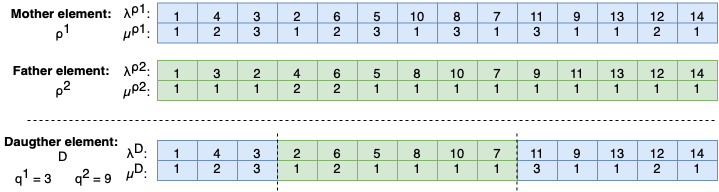
\includegraphics[width=0.93\textwidth]{assets/img/04_Umsetzung/TwoPointCrossover.drawio.png}
    }
    \caption{Beispiel des Two-Point Crossover für das MRCPSP} 
    \label{img:twopointcrossover}
    \source{Eigene Darstellung}
\end{figure}


\subsubsection*{Umsetzung des Mutation Operator}

Der implementierte Mutation Operator soll innerhalb der Aktivitäts- und Moduslisten von Nachfahren $\lambda$ leichte Änderungen realisieren. Tupels von austauschbaren Aktivitäten werden hierbei jeweils mit einer Wahrscheinlichkeit von $p_{mutation} = \sigma$ miteinander vertauscht. Mit der selben Wahrscheinlichkeit $\sigma$ zudem wird für jede Aktivität erneut ein zufälliger Modus selektiert. \\

Die Wahl einer optimalen Mutationsrate $\sigma$ stellt eine Herausforderung dar. Die Rechenberg Regel modifiziert die Mutationsrate $\sigma$ in Abhängigkeit der Erfolgsrate einer Population. Bei einer Erfolgsrate von weniger als 1/5 wird die Rate erhöht, bei 1/5 bleibt die Mutationsrate gleich. Sofern die Erfolgsrate größer als 1/5 ist, wird die Mutationsrate erhöht. \cite[vgl.][S. 24 f.]{kramer_genetic_2017} \\

Eine abgewandelte Form der Rechenberg Regel wird für den umgesetzten Algorithmus verwendet. Für die Implementierung bezieht sich die Erfolgsrate auf die Verbesserung des besten Individuums. Eine Population, die das neue beste Individuum gemäß der Fitness beinhaltet, wird als erfolgreich angesehen. Die Mutationsrate $\sigma$ wird über die folgende Formel geändert:
\begin{align*}
    \sigma = \sigma * \exp^{0.05}(a - \tfrac{1}{5}) && \text{mit }a = \begin{cases}
    0 & \text{mit Erfolgsrate} < 1/5 \\ 
    1 & \text{mit Erfolgsrate} \geq 1/5 \\ 
    \end{cases}
\end{align*}

\subsubsection*{Umsetzung des Selection Operator}
Bei dem implementierten Algorithmus handelt es sich um ein $(\mu+\lambda)-GA$, wobei die Lebensdauer einer Lösung auf $\kappa$ Generationen beschränkt ist. Wenn somit ein Individuum über $\kappa$ Generationen in die kommenden Population ausgewählt wurde, so wird die Lösung nicht mehr in der kommenden Population selektiert werden können. Es gilt das Individuum zu selektieren, für welches der Wert der Fitnessfunktion $f(x)$ am geringsten ist. 

\subsubsection*{Umsetzung der Fitnessfunktion}
Die umgesetzte Fitnessfunktion $f(x)$ orientiert sich an den Definitionen und der Priorisierungen der Zielfunktionen aus Abschnitt \ref{sec:AuswahlMetaheuristischenAlgorithmen}. Dadurch resultiert eine weitaus stärkere Gewichtung der Projektdauer $C_{max}$ im Vergleich zur Robustheit $\Omega$. Die Fitnessfunktion $f(x)$ ist gemäß dieser Gewichtung über die folgende Formel definiert:
\begin{align*}
f(x) = C_{max}(x) - \dfrac{\Omega(x)}{100}
\end{align*}
